%!TEX root = main.tex
\section{Architecture}
\label{sec:architecture}

This section describes the architecture of the \sys prototype, depicted in \autoref{fig:architecture}, as well as providing some additional implementation details (\S\ref{ssec:impl}).
%In this chapter, the implementation of the main application, whose main role is to  orchestrate the execution of the various benchmarks across the cloud providers. 
%We provdie an overview of the varius compoentns and functionalities the components and their functions will be briefly explained and later every main task the user can do will be explained in detail.
%\subsection{Overview}
The architecture includes the supported clouds and the corresponding serverless services (left), the involved Docker images (middle) and their interface with the system (right).
We detail each component next. 

\begin{figure}[!t]
\begin{center}
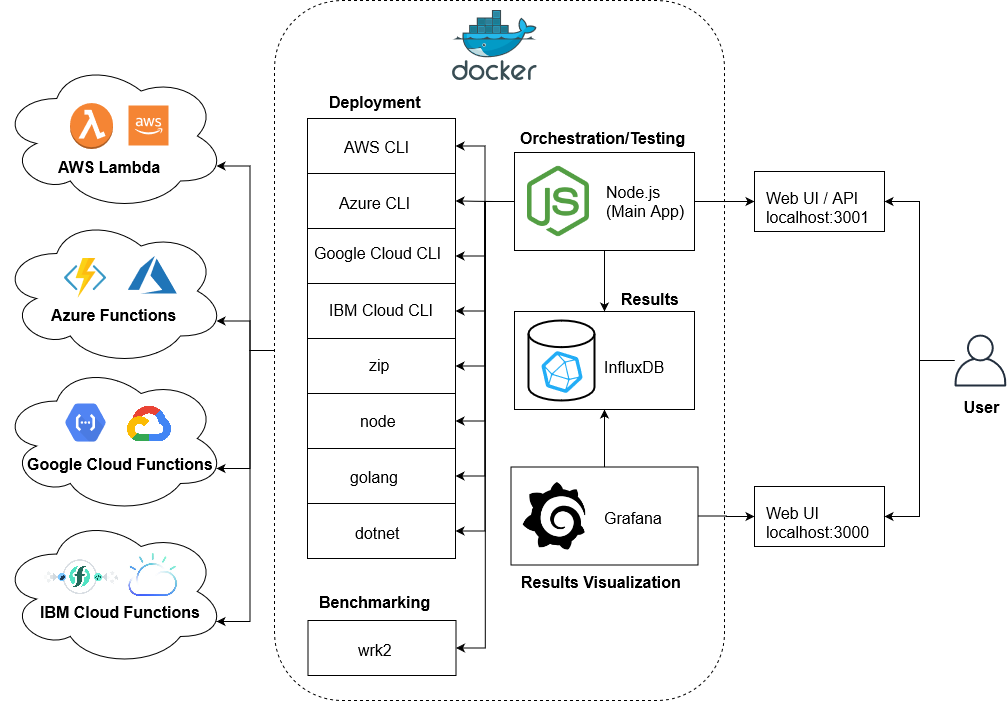
\includegraphics[width=0.45\textwidth]{bilder/main_app.png}
\caption{\sys architecture.}
\label{fig:architecture}
\end{center}
\end{figure}



\textbf{Main application.} The \sys core component is implemented in JavaScript and leverages the Node.js framework. 
It manages all user input and executes the actions or delegates them to other components. 
This application is packaged and executed as Docker containers. 
%Only the Linux packages \texttt{docker-ce} and \texttt{docker-compose} are needed to execute this program. 
%Figure \ref{fig:architecture} depicts all components and gives an overview of the \sys suite.
It manages the following main tasks: \emph{(1)} deployment to the clouds, \emph{(2)} execution of tests benchmarks, \emph{(3)} computing price estimations. 
Users access it through a web \gls{GUI} or via a REST \gls{API}. 
Once started, the set of configured tests are deployed (some examples given in Section~\ref{sec:tests}) to be executed.
%After the tests are deployed, they can be tested and benchmarked. 

\textbf{Time Series DB:} a time-series database, where all the results from tests are be stored and later on used by graphical interfaces and pricing calculation. Our prototype uses InfluxDB~\cite{influx}.

\textbf{UI:} the architecture provides an API to easily integrate visualization tools. Our prototype integrates with Grafana~\cite{grafana}, an open source tool to display, plot and monitor data stored in a database. 
The results gathered by the tests and stored in InfluxDB will be displayed in Grafana.

\textbf{CLIs:} With the exception of AWS, all cloud providers offer a Docker image for their \gls{CLI}. 
Resources can be deployed, deleted and managed completely by the \gls{CLI}.

\textbf{Runtimes (Node.js, Go, .NET):} In addition to the source code of the function(s) to execute, a built and packaged zip file is commonly required to successfully complete the deployment. 
The \sys architecture allows developers to ship runtime images, fo instance used to install packages and build or run the corresponding sources.

%\vs{to remove:
%\textbf{zip:} this image zips the files that need to be deployed to the clouds. 
%Therefore there is no need to have zip installed on the machine the benchmark suite runs.
%}

\textbf{Workload Injectors}. The architecture provides hook points to plugin workload injectors. The evaluation results shown in Section~\ref{sec:evaluation} uses \texttt{wrk2}~\cite{wrk2}, a stress tool for REST services. \sys uses it to issue requests toward services and gather throughput/latency results.

%%%MOVE TO GITHUB/README
%%%\subsection{Requirements}
%%%\vs{I would move this section completely and have these details in the github/readme page}
%%%To use this application, there are some prerequisite steps necessary. 
%%%First of all, the user needs to have or create accounts on the clouds he intends to test on. 
%%%%This process will be not described in detail since it is straightforward to do. 
%%%%There is however a small guidance for each cloud provider in the documentation on GitHub.\\
%%%Secondly, the user needs to have a Docker environment installed. 
%%%%This is not too difficult on Linux and described exemplary for Ubuntu 18.04 on GitHub.\\
%%%After these steps have been completed some more manual initialization and configuration steps are required from the user. 
%%%He needs to create a few Docker volumes and perform the login process for each \gls{CLI} belonging to the cloud intended to be tested.\\
%%%As last point some free storage is required because some Docker images are quite large, in total around 5.15 GB. 
%%%In addition, some free space should be reserved for the data that will be stored in the database, 1 GB should be sufficient. Table \ref{table:images} shows all images and their sizes.
%%%\begin{table}[htp]
%%%\centering
%%%\captionsetup[table]{justification=centering, labelfont=bf}
%%%\begin{tabular}{|l|l|r|}\hline
%%%\textbf{Repository} & \textbf{Tag} & \textbf{Size} \\ \hline
%%%bschitter/benchmark-suite-serverless-computing	&	0.1	&	358MB	\\ \hline
%%%mikesir87/aws-cli	&	1.16.310	&	186MB	\\ \hline
%%%google/cloud-sdk	&	274.0.1-alpine	&	287MB	\\ \hline
%%%mcr.microsoft.com/azure-cli	&	2.0.78	&	1.04GB	\\ \hline
%%%mcr.microsoft.com/dotnet/core/sdk	&	2.2-alpine3.9	&	1.48GB	\\ \hline
%%%bschitter/alpine-with-zip	&	0.1	&	6.32MB	\\ \hline
%%%bschitter/alpine-with-wrk2	&	0.1	&	232MB	\\ \hline
%%%ibmcom/ibm-cloud-developer-tools-amd64	&	0.20.0	&	309MB	\\ \hline
%%%golang	&	1.11-stretch	&	757MB	\\ \hline
%%%node	&	10.16.2-alpine	&	76.4MB	\\ \hline
%%%grafana/grafana	&	6.3.2	&	254MB	\\ \hline
%%%influxdb	&	1.7.7-alpine	&	137MB	\\ \hline
%%%\textbf{Total size} & & \textbf{5.15GB}\\ \hline
%%%\end{tabular}
%%%\caption[Docker images]{Docker images}
%%%\label{table:images}
%%%\end{table}

\begin{figure}[!t]
\begin{center}
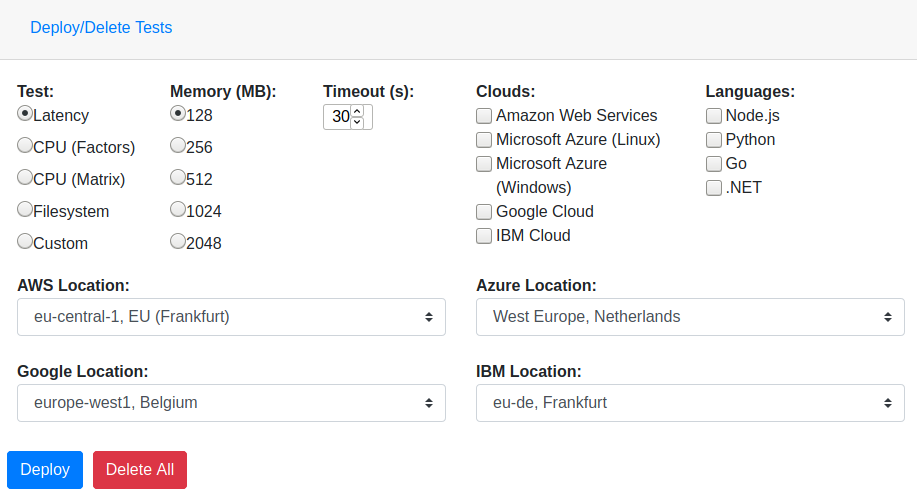
\includegraphics[width=0.45\textwidth]{bilder/ui.png}
\caption{\sys: web GUI}
\label{fig:ui}
\end{center}
\end{figure}

\subsection{Deployment}
%This section will describe the deployment process of the tests.
Once the main application has started, the client can deploy the desired tests, for instance via the web-based interface shown in Figure~\ref{fig:ui}.
Functions can be parametrized with memory allocated \mais{per single execution, to each instance not each execution}, timeouts, which serverless providers to use for the benchmarks, which runtime version to use, and into which geographical regions (as supported by the cloud provider) to deploy the tests. 
%\begin{itemize}
%    \item \textbf{Test:} a unique identifier for the test to execute to deploy;
%    \item \textbf{Memory:} The amount of memory to allocate per function.\footnote{Azure assignmes memory dynamically, up to 1536 \gls{MB} per function}
%    \item \textbf{Timeout:} The time limit after which a running function will time out. %\\ \textbf{Remark:} Not applicable for Azure since it handles timeout configuration in a configuration file.
%    \item \textbf{Clouds:} The cloud providers the tests will be deployed on, multiple choices possible.
%    \item \textbf{Languages:} Runtimes respectively languages to deploy the function in, multiple choices possible.
%    \item \textbf{Locations:} The region where the function will be deployed to.
%\end{itemize}
Once deployed, the interface continuously reports on the progress and potential issues (\emph{e.g.}, timeouts, access problems, etc.). 
%Next the \textit{Deploy} button can be pressed and the application will initiate the deployment. On the right hand side of the web interface there will be information about the progress. 
The deployment process is parallelized, including the creation of the required cloud resources, building and packaging the functions, as well as their upload over the cloud.
The deployment flows are slightly different for each provider. 
Figure~\ref{}\vs{FIX} illustrates the various steps for those supported by \sys.
\vs{MAISSEN: I've looked a the flowcharts in the appendix of the report. Apart from the google one which seems very simplistic, I wonder if we could have a figure combining those ones into a figure that we could report here in the deployment section. ... flow charts are illustrating the deployment and cleanup process for each cloud.} \mais{Yes I can try to combine and minify them. Maybe I forget about the runtime differences (build, zip) and only illustrate the essentail 'cloud' part?}\vs{YES :-) Figure should be very minimalistic, to span only 1 column possibly. Use PDF/EPS format - although we might want to tune the figs somehow later one}

\subsection{Testing}
%In this section it is briefly explained how to execute a test and see its results. 
The test will send every five seconds a request to the functions previously deployed, with the purpose to gather baseline results under low, constant load. %As options, a name for the test and the functions parameter can be set. 
Figure~\ref{fig:grafana} illustrates a screenshot of Grafana showing test results of a latency test in Node.js. 
%At the top, there are three drop down menus to choose the test type, the test name (given at the start of the test) and the data points interval.

\begin{figure}[!t]
\begin{center}
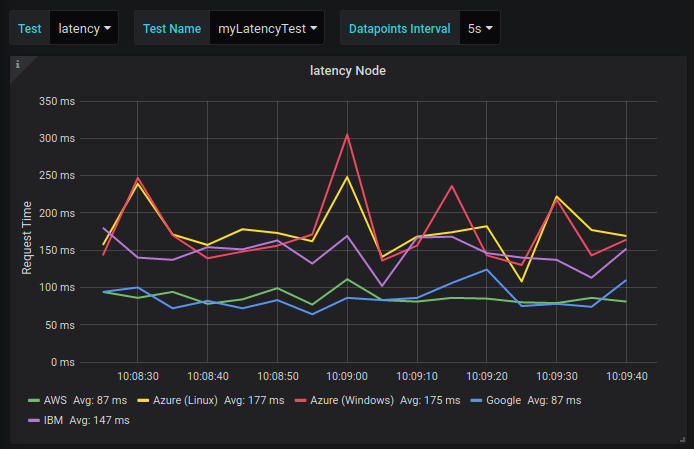
\includegraphics[width=0.45\textwidth]{bilder/grafana.png}
\caption{Visualization of performance results in Grafana}
\label{fig:grafana}
\end{center}
\end{figure}

%The plots can be grouped by cloud provider or by runtime. 
%There is a predefined Grafana dashboard for both options, the user can switch depending on his interests. 

%An example result of a general test can be seen in section \ref{sec:general_test}.

\begin{figure*}[!t]
\begin{center}
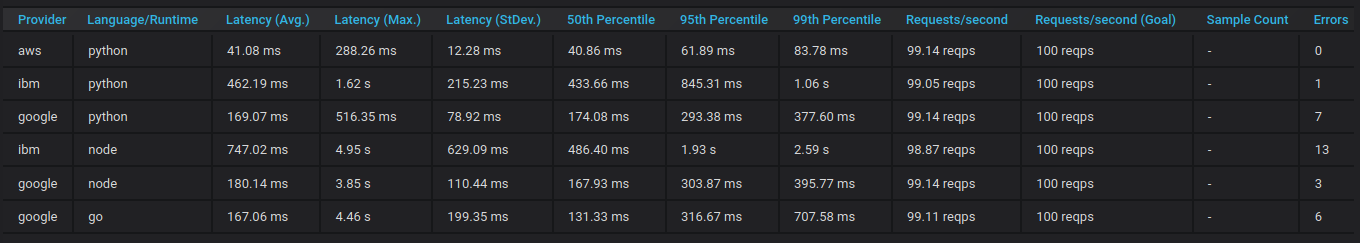
\includegraphics[width=1\textwidth]{bilder/benchmark_table.png}
\caption[Benchmark results in Grafana]{Benchmark results in Grafana.}
\label{fig:benchmark_table}
\end{center}
\end{figure*}


\subsection{Benchmarking}
The benchmarking component injects specific workloads toward a function exposed by a given serverless provider.
Our design is modular and currently supports \sloppy{\texttt{wrk2}~\cite{wrk2}}, a constant throughput/correct latency HTTP benchmarking tool. 
Additional tools are easy to integrate by providing a Docker container and a simple REST interface to exchange parameters and results. 
\sys architecture allows to directly visualize and analyze these results, for instance using Grafana (Figure~\ref{fig:grafana}).
%mainly relies on the wrk2 image. The parameters can be set in the web interface but they are basically just forwarded to wrk2. For the benchmark itself the user can choose the following parameters: requests per second, duration of the benchmark and the desired test to run e.g. the \gls{CPU} factors test. 
%Afterwards the load test will start and benchmark the chosen function on each cloud and runtime it was deployed to. 
%This process has to run sequentially otherwise the host of the benchmark suite could potentially not handle the load. 
%After the test has completed results will be parsed and inserted into the database and can be viewed as a table in Grafana. Figure \ref{fig:benchmark_table} shows an excerpt of a result.

\subsection{Cleanup}
Upon cleanup, all deployed Lambda \mais{omit Lambda or use serverless} functions are permanently deleted, as well as all the configurations and resource groups created at deployment time. % and \gls{API} gateways on \gls{AWS} and IBM, all resource groups with a name containing latency, factors, matrix, filesystem and custom and on Google all functions in the configured project. 
%It should therefore be used very carefully and ideally with separate accounts only for this purpose.



%A more detailed test example with increasing load is discussed in section \ref{sec:loadtest}.

\subsection{Billing Costs Calculator}\label{ssec:billingcalc}

The core component embeds a pricing calculator, which can be used to calculate beforehand the cost of executing a certain workload on the supported cloud providers. 
%It does so either by setting the corresponding parameters manually or by exploiting results from previous executions.
%This component can be used to predict the cost of executing a given benchmark on a specific cloud provider.
Developers provide the planned workload (\eg number of function invocations, execution time per call, size of the return body and allocated memory, \etc).
The \sys prototype produces an overview of the billing costs across the various serverless providers.
In future work, we envision this module to be able to forecast the billing costs even for full-fledged serverless applications, by applying machine-learning techniques to the system traces produced by sampling executions serving real-world workloads.
%The prices for all clouds will be calculated and displayed in a table. 
%The functionality is basically the same as the pricing calculators provided by the cloud providers, except here all is in one place and directly comparable.
%Furthermore, the calculator takes the performed tests into account. 
%One can select a previously run test, select a runtime and then one only needs to provide the estimated number of invocations per month. 
%The calculation will happen by taking the execution time from the test results which of course can vary quite a lot between cloud providers and runtimes. 
%This method allows a much better approach of estimated cost. 
%In section \ref{sec:pricing} the same example will be explained and calculated for both hypothetical and with actual test results as input.

\subsection{Implementation Details}\label{ssec:impl}
The implementation of \sys rely on Docker containers.
Specifically, the main container must invoke other containers, using a technique called \emph{Docker-in-Docker}.\footnote{\url{https://www.docker.com/blog/docker-can-now-run-within-docker/}}
We do so by granting access to the main container to \texttt{/var/run/docker.sock}, \emph{i.e.} mounting it as volume.
During our evaluation, we did not observe specific performance degradations using this approach.

The implementation of \sys is freely available to the open-source community at \url{https://github.com/faasdom/benchmark-suite-serverless-computing}, and it consists of about 2000 lines of Node.js code.